\chapter{Introduction}\label{ch:introduction}

Complex systems are common in both nature and society and are closely related to our daily lives. Many significant large-scale phenomena, such as climate change, forest fires and pandemics, can be understood and studied as complex systems. In general, a complex system can be described as a large, coupled, nonlinear spatial system in which components interact with each other. Because of these interactions, the macroscopic behaviour of the system can be difficult to recognise from the microscopic model \cite{Fieguth2021}. 

This report will focus on self-organised criticality (SOC) and the associated non-Gaussian statistics in complex systems. In particular, I will use the Bak–Tang–Wiesenfeld (BTW) sandpile model, a representative model exhibiting self-organised criticality.

\par\vspace{0.5cm}
\noindent
\noindent\hspace*{0.08\textwidth}
\begin{minipage}[t]{0.32\textwidth}
    \centering
    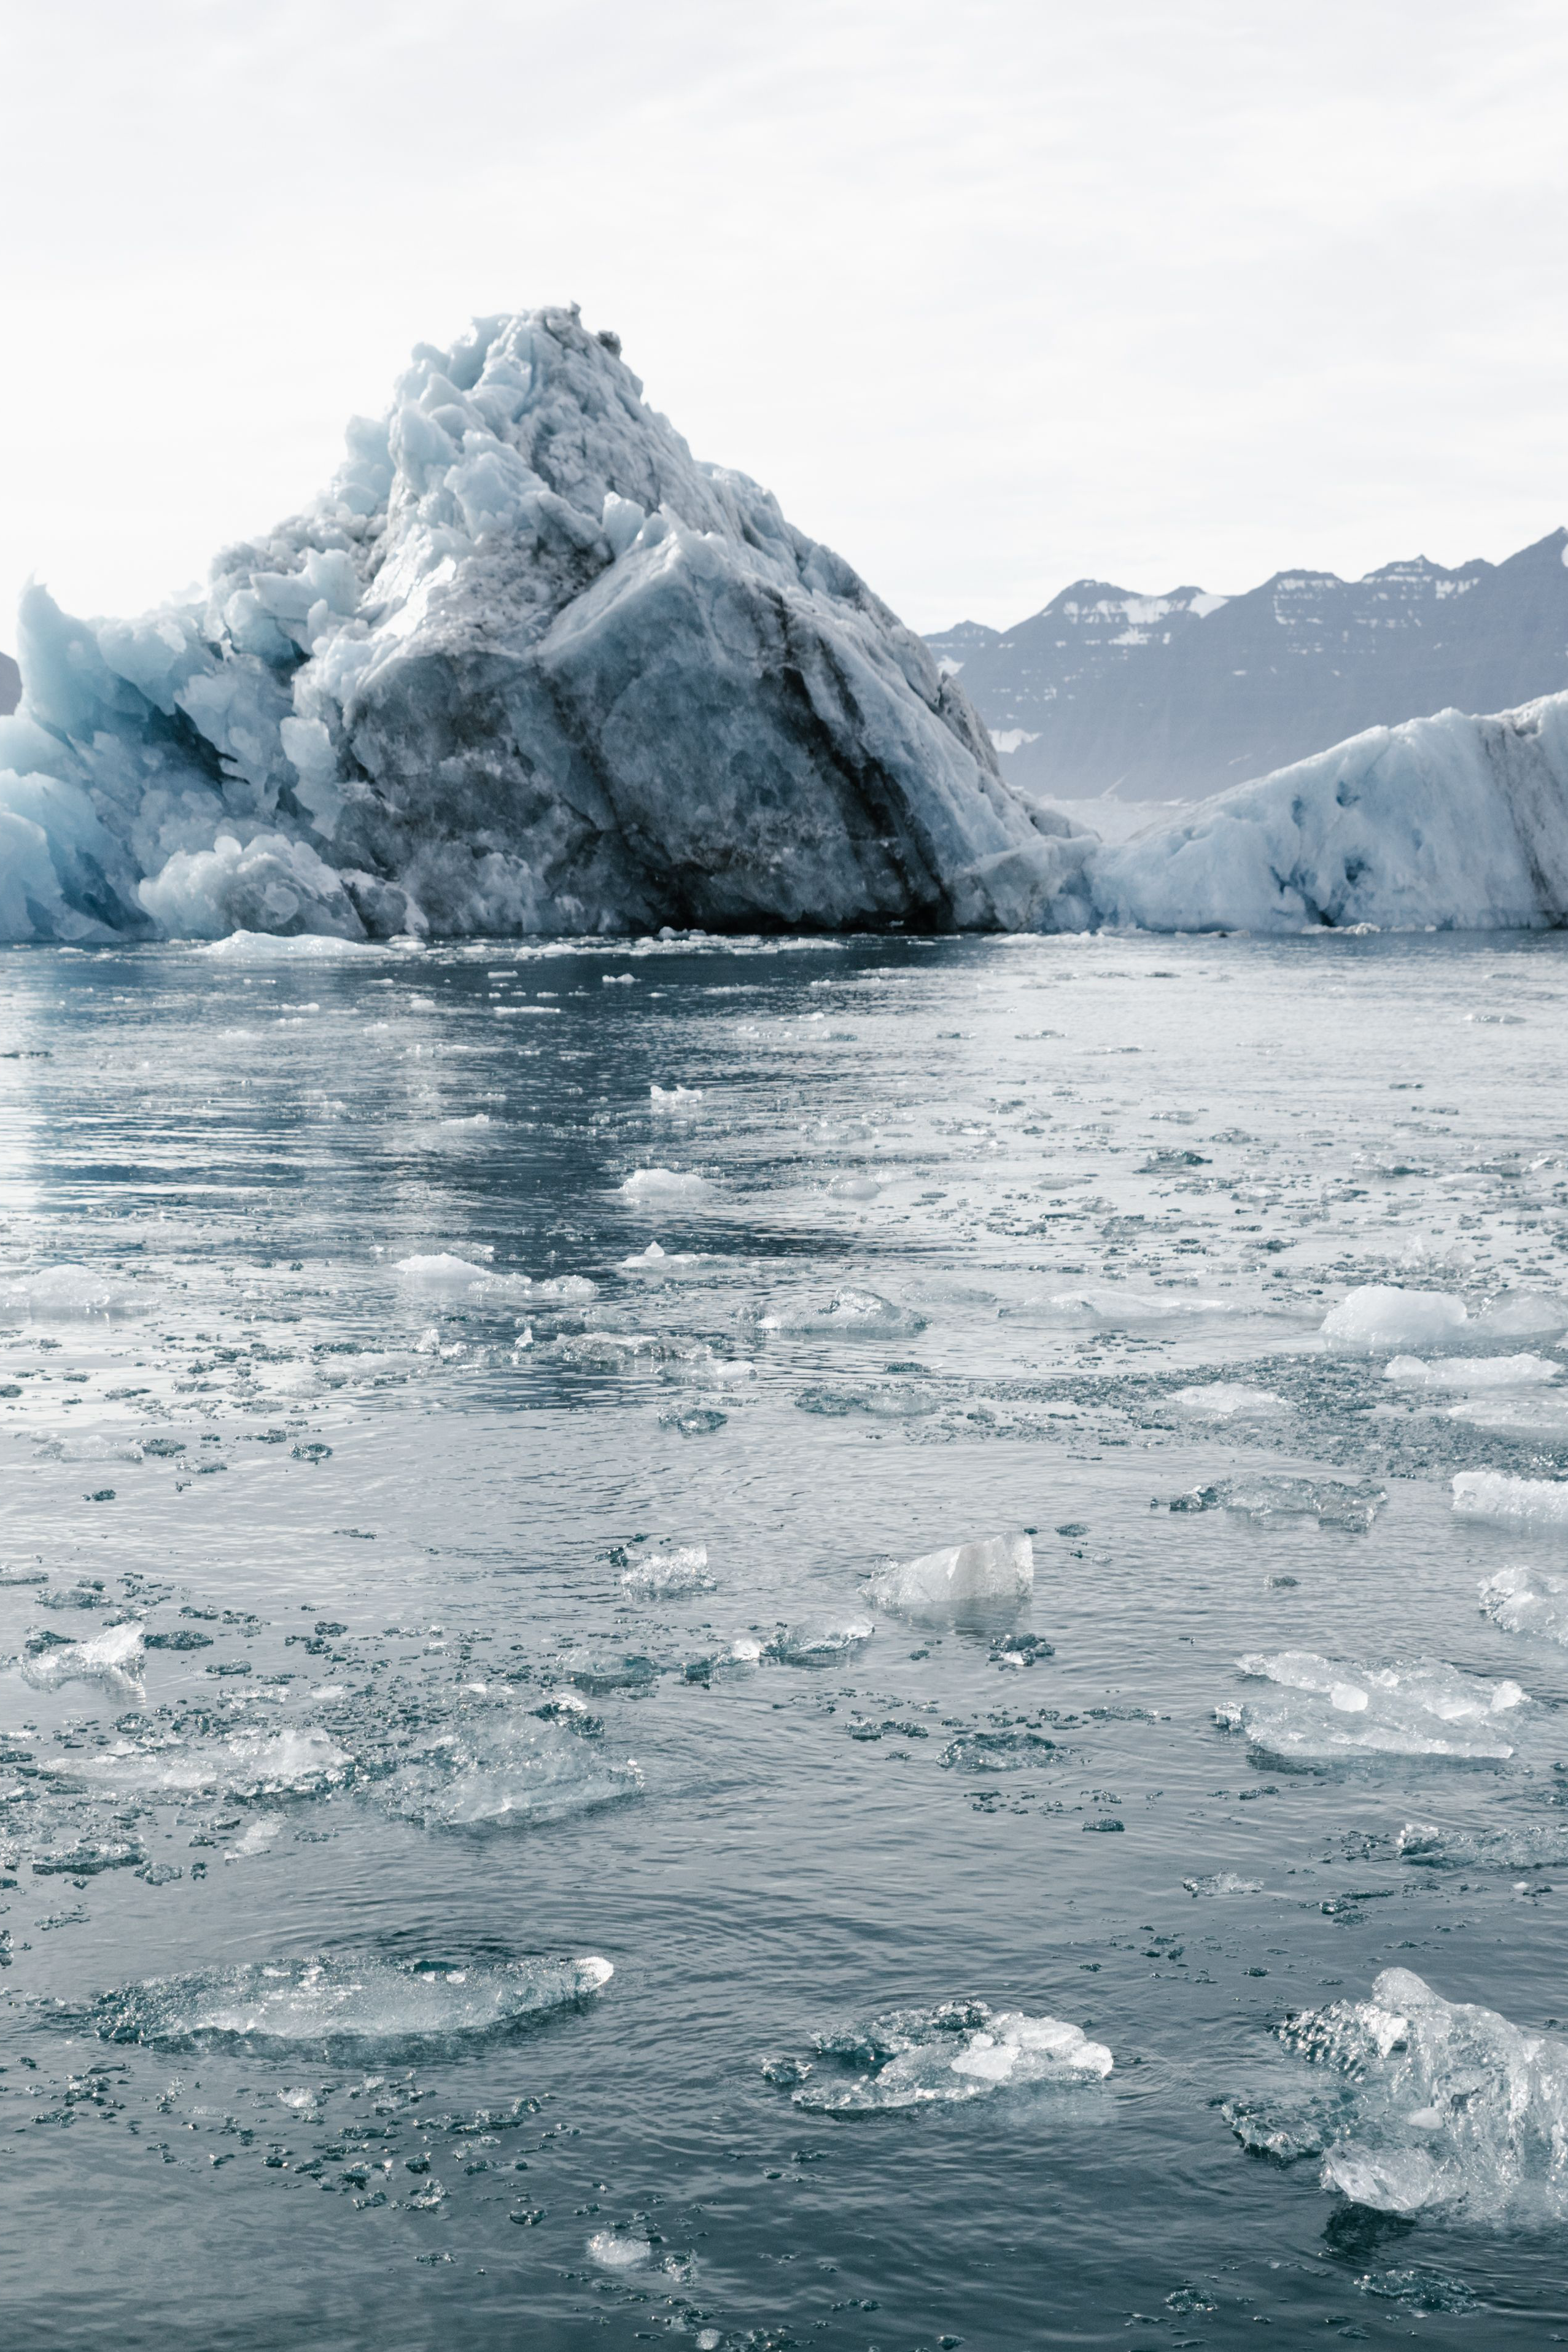
\includegraphics[width=\linewidth,height = 9cm]{figures/iceberg.jpg} \captionsetup{format=plain,justification=raggedright,singlelinecheck=false}
    \captionof{figure}{A melting iceberg in Arctic waters \cite{ArtHouseIceberg}.}
    \label{fig:iceberg}
\end{minipage}%
\hspace{0.12\textwidth}%
\begin{minipage}[t]{0.32\textwidth}
    \centering
    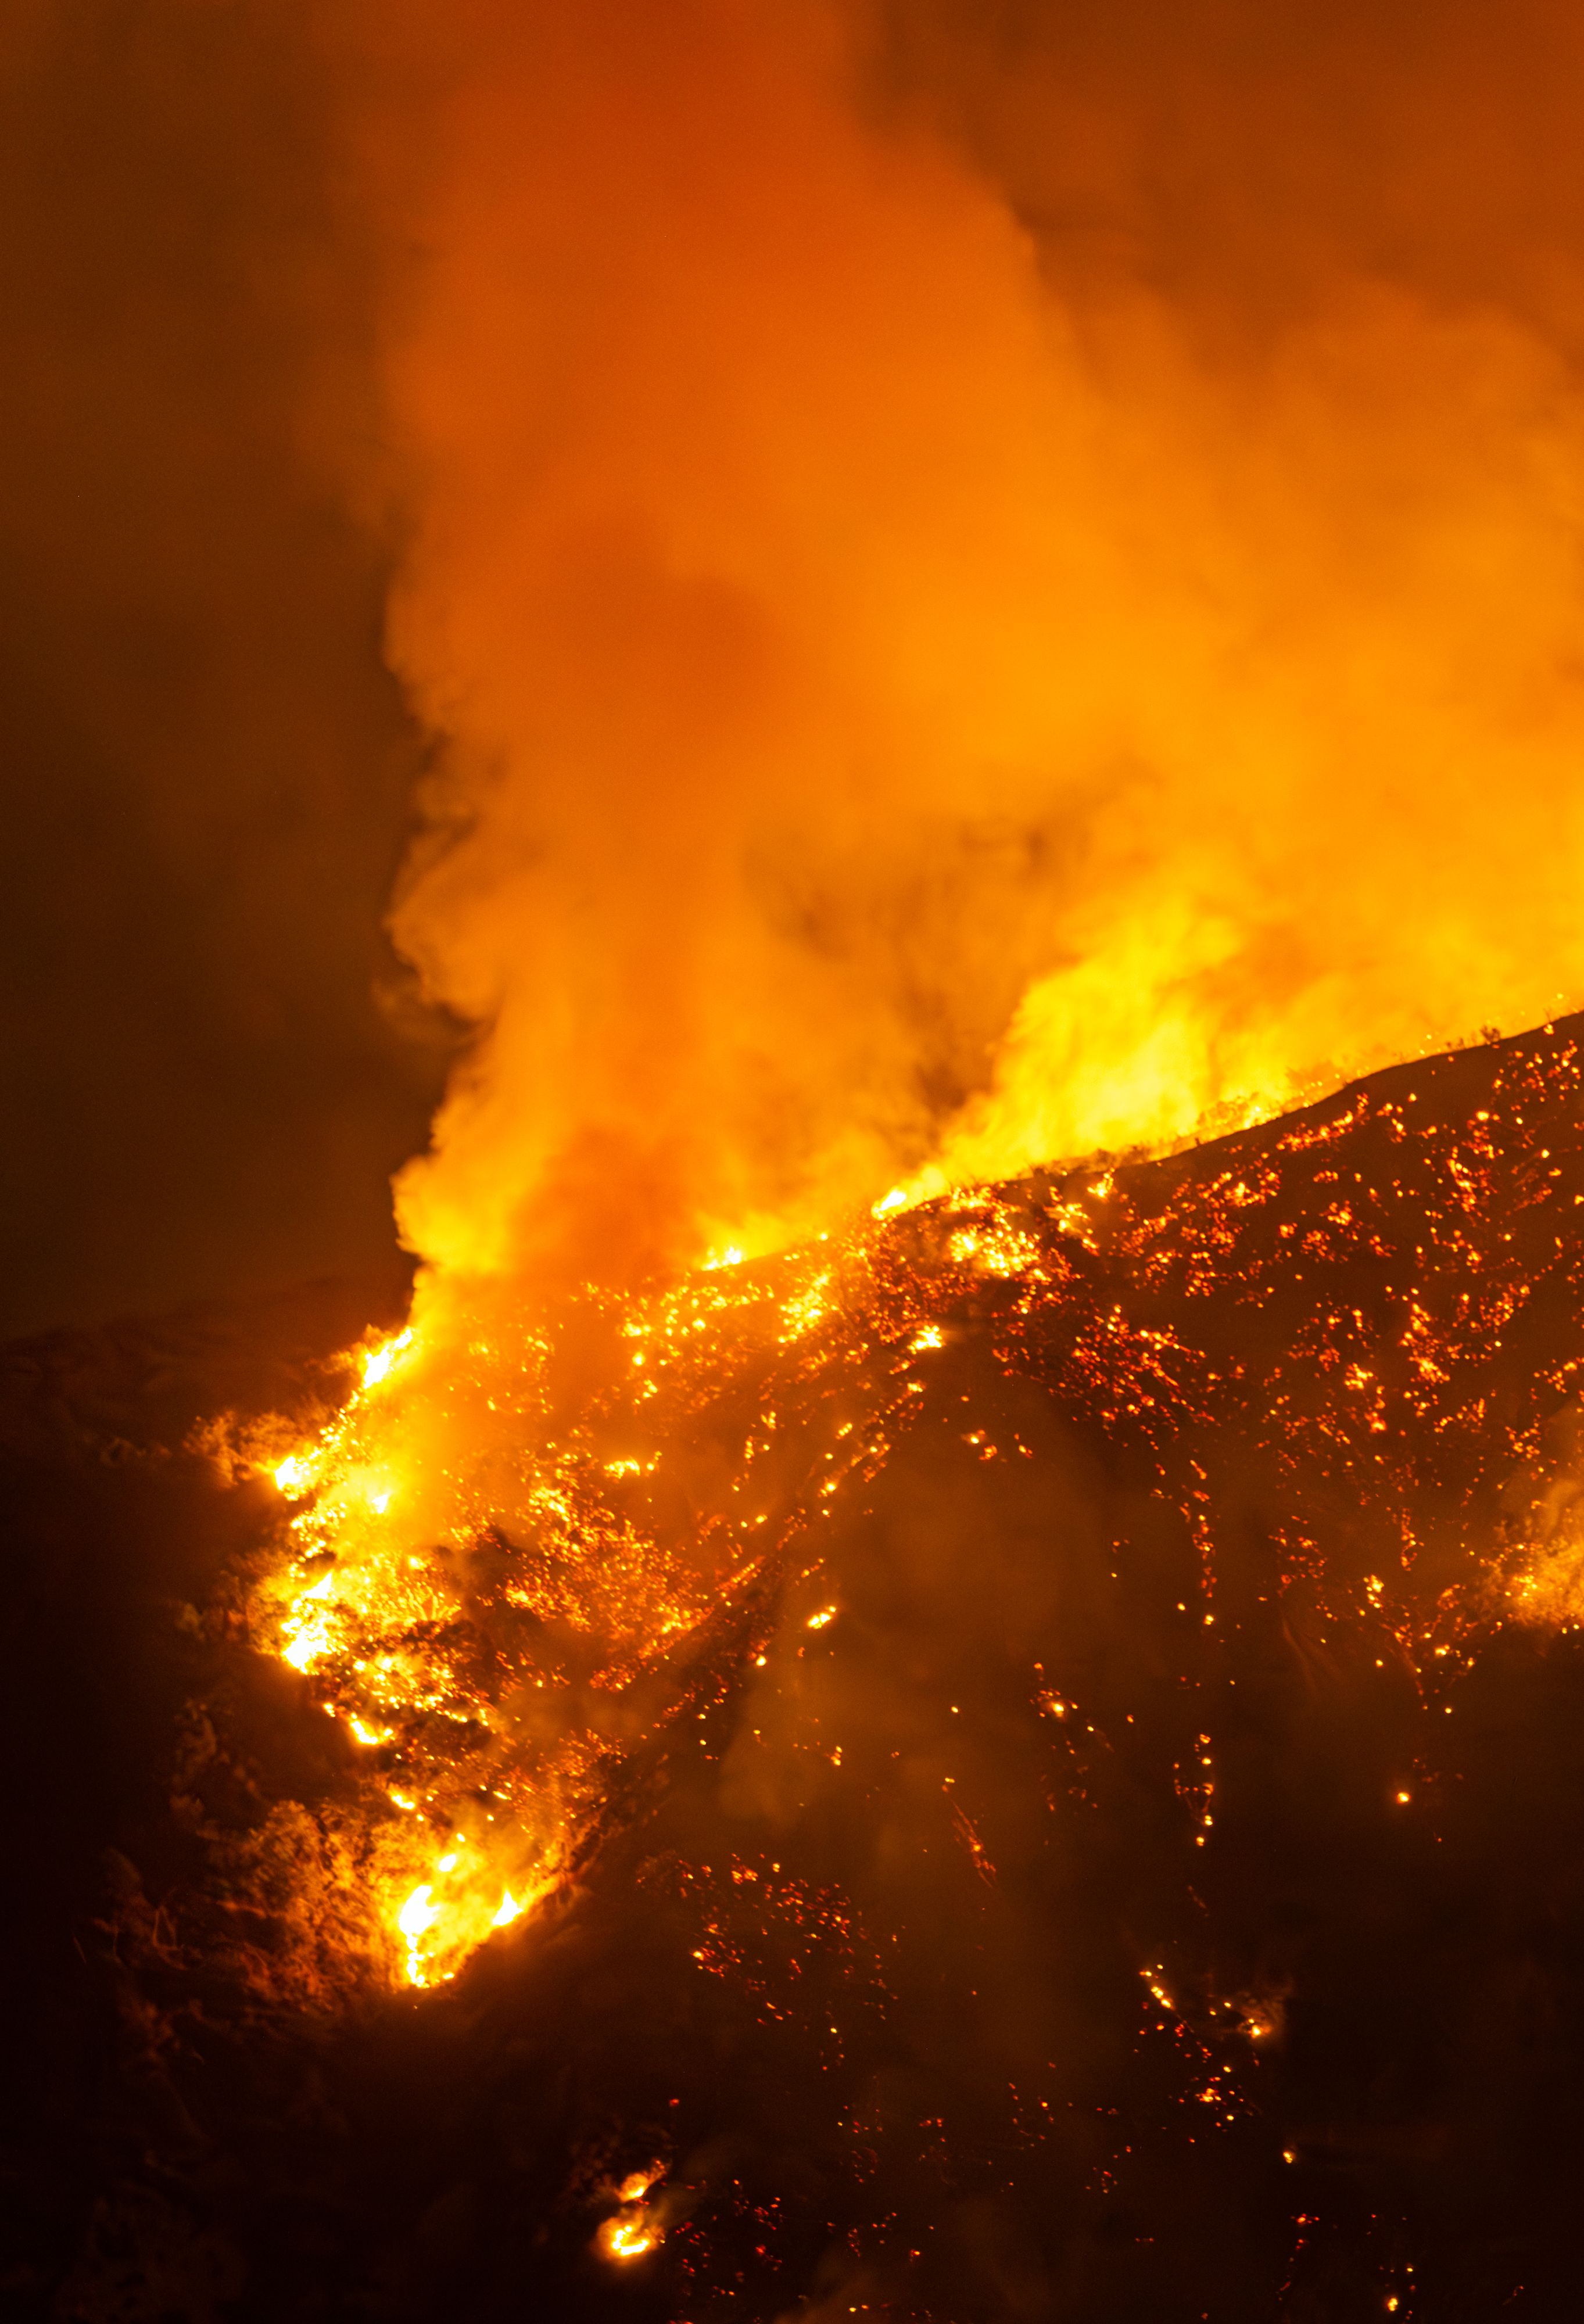
\includegraphics[width=\linewidth,height = 9cm]{figures/wildfire.jpg} \captionsetup{format=plain,justification=raggedright,singlelinecheck=false}
    \captionof{figure}{A wildfire in California \cite{MosesWildfire}.}
    \label{fig:wildfire}
\end{minipage}
\par


\section{Self-Organised Criticality (SOC) and Scale Invariance}

According to the research of Bak, Tang, and Wiesenfeld, dynamical systems with extended spatial degrees of freedom naturally evolve into a self-organised critical state, which is barely stable. In such a state, small perturbations at a certain location may render the neighbouring sites unstable, and the perturbations may spread to the neighbours in a chain reaction \cite{Bak1987}. Self-organised means that the system can naturally evolve to the critical state without detailed specification of the initial conditions. A critical state is a state with no characteristic time or length scales, exhibiting scale invariance \cite{Bak1988}.

\begingroup
\renewcommand{\thefootnote}{}
\footnotetext{The cover image was generated using WebGL Sandpiles: \url{https://people.reed.edu/~davidp/web_sandpiles/}.}
\endgroup

\newpage

Scale invariance is usually defined as the structure or property of a system remaining unchanged as the scale changes. Mathematically speaking, it can be described as $$f(\lambda x) = C(\lambda) f(x)$$
for $\lambda > 0$, where $C(\lambda)$ is the scaling factor that does not depend on $x$ \cite{Khaluf2017}. This relation means that multiplying the input by a factor of \(\lambda\) preserves the functional form, while multiplying the output by a corresponding factor of \(C(\lambda)\). This requirement constrains the functional form to a power law, usually written as $f(x) = Ax^\alpha$, where \(A\) and \(\alpha\) are constants. This explains why phenomena in systems exhibiting scale invariance can be described by power laws  \cite{Newman2005, Sornette1998}.

\section{Bak–Tang–Wiesenfeld (BTW) model}

The Bak–Tang–Wiesenfeld (BTW) sandpile model was introduced by Per Bak, Chao Tang and Kurt Wiesenfeld to explain self-organised criticality \cite{Bak1987}. The BTW sandpile model is selected in this project because its simple local rules can lead to complex collective behaviour through interactions between sites. 

In particular, the model consists of a two-dimensional grid of a chosen size. At each step, a grain of sand is added to a randomly chosen grid point. If the number of grains at a grid point reaches or exceeds four, the site topples, transferring one grain to each of its four nearest neighbours. Any grains that fall outside the grid are removed from the system. A new grain is added only after all toppling activity has ceased. 

The model has extended spatial degrees of freedom, as each site of the two-dimensional grid has its own state, represented by the number of sand grains at that site. According to the toppling rule, a topple at one site affects its neighbours and may trigger further toppling, leading to a chain reaction. Additionally, sand addition, toppling, and open boundaries allow the system to self-regulate the accumulation and loss of sand grains, eventually reaching a state where average input balances average loss. This process illustrates how the system regulates itself without external fine-tuning. In the resulting state, the distribution of avalanche area exhibits approximate power-law behaviour, indicating scale invariance and criticality \cite{Bak1987}.


\begin{figure}[htbp]
    \centering
    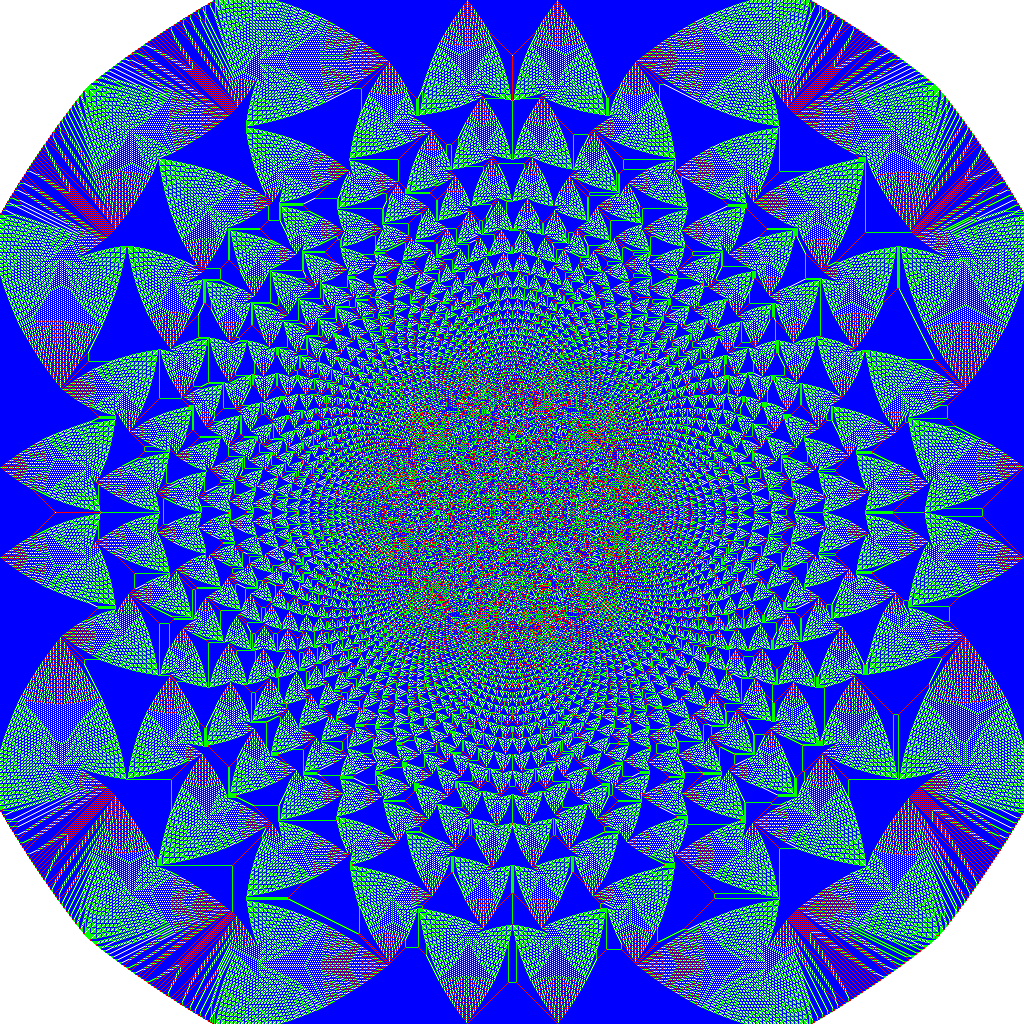
\includegraphics[width=0.5\textwidth]{figures/model.jpg}
    \caption{A BTW sandpile pattern in which the sand
    was dropped continuously onto the centre \cite{Rocchini2012}.}
    \label{fig:btw-pattern}
\end{figure}
\section{Aim}
This project aims to study SOC and the associated non-Gaussian statistics in the basic BTW sandpile model, and to compare this model with a gradient-dependent extension. In particular, this project will mainly focus on investigating the steady-state behaviour of the basic model, analysing the distributions and correlations of four avalanche properties and examining the mathematical properties of the toppling rules. The behaviour and avalanche statistics of the basic model will then be compared with the gradient-dependent extended model.
